\documentclass[12pt]{article}

\usepackage[T1]{fontenc}
\usepackage[utf8]{inputenc}
\usepackage[icelandic]{babel}
\usepackage{setspace}
\usepackage{comment}
\usepackage{wrapfig}
\usepackage{listings}
\usepackage{courier}
\usepackage{verbatim}
\usepackage{tikz}
\usepackage{caption}
\usepackage{gensymb}
\usepackage{hyperref}
\usepackage{gensymb}


\usepackage{xcolor}
\definecolor{commentgreen}{RGB}{2,112,10}
\definecolor{eminence}{RGB}{108,48,130}
\definecolor{weborange}{RGB}{255,165,0}
\definecolor{frenchplum}{RGB}{129,20,83}

%\usepackage{minted}

\lstdefinestyle{customc}{
  belowcaptionskip=1\baselineskip,
  breaklines=true,
  frame=L,
  xleftmargin=\parindent,
  language=C,
  showstringspaces=false,
  basicstyle=\footnotesize\ttfamily,
  keywordstyle=\bfseries\color{green!40!black},
  commentstyle=\itshape\color{purple!40!black},
  identifierstyle=\color{blue},
  stringstyle=\color{orange},
}

\lstdefinestyle{customasm}{
  belowcaptionskip=1\baselineskip,
  frame=L,
  xleftmargin=\parindent,
  language=[x86masm]Assembler,
  basicstyle=\footnotesize\ttfamily,
  commentstyle=\itshape\color{purple!40!black},
}

\lstset{style=customc,captionpos=t}



\captionsetup{labelformat=empty}

\usepackage{amsmath,amssymb,graphicx,color,enumerate,here}
\setlength{\parindent}{0cm}\newcommand{\Z}{\mathbb{Z}}\newcommand{\R}{\mathbb{R}}\newcommand{\C}{\mathbb{C}}
\newcommand{\N}{\mathbb{N}}\newcommand{\f}[2]{\frac{#1}{#2}}\newcommand{\1}[1]{\frac{1}{#1}}

\voffset=-1.0in
\hoffset=-0.3in
\textwidth=6in
\textheight=9in

\begin{document}
\noindent \large \textbf{Verkefni 2 \hfill Jónas G. Sigurðsson\\
\noindent Tölvugrafík \hfill 
\normalsize  \hfill mars 2019}\\\\
\begin{small}

\begin{spacing}{2}
\end{spacing}

Einstaklingsverkefni 2 snérist um að búa til þrívítt fiskabúr með 10 fiskum, sem hver og einn syndir í slembiátt og á slembihraða og þeir birtast á slembistað í búrinu. Ef að fiskarnir synda á vegg þá birtast þeir hinu megin í búrinu.\\

Í minni lausn eru fiskarnir einnig í slembilitum, einn fyrir búk, einn fyrir ugga og einn fyrir sporð og þeir hreyfa uggana og sporðana óháð hvor öðrum og ekki í takt.
\begin{center}
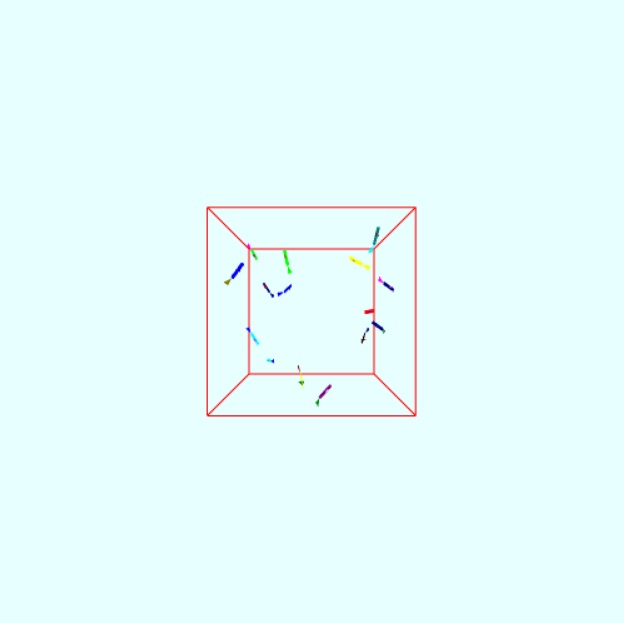
\includegraphics[scale=0.5]{1}
\end{center}
Hægt er að halda vinstri músarhnapp inni og hreyfa búrið til með því að draga músina til. Möguleiki er á því að þysja inn og út með því að nota upp/niður örvar.
\begin{center}
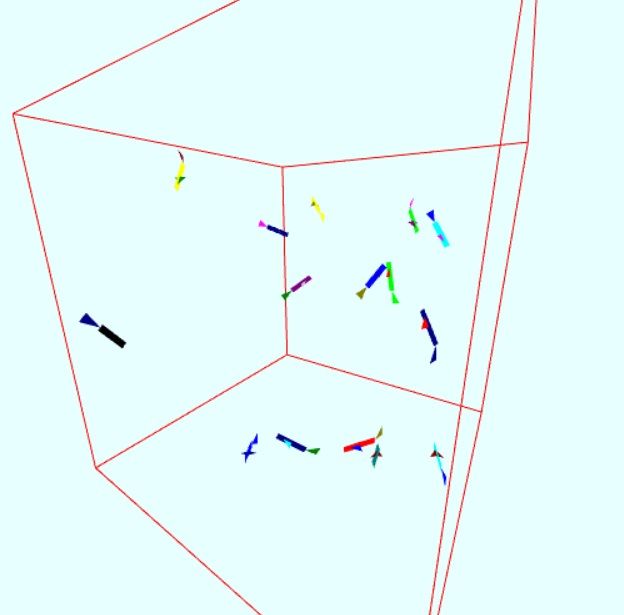
\includegraphics[scale=0.5]{2}
\end{center}
Ef ýtt er á "A" hnapp þá laga fiskarnir sundstefnuna sína og hraða að hópnum og fara að synda í sömu átt eftir nokkrar sekúndur.
\begin{center}
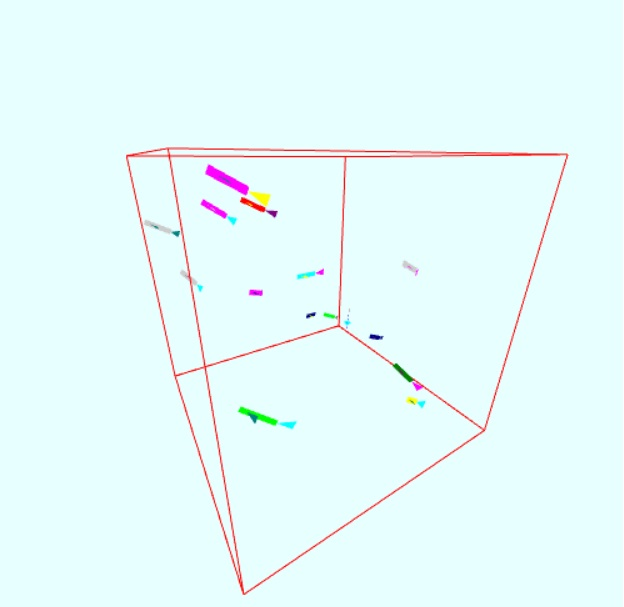
\includegraphics[scale=0.5]{3}
\end{center}
Lausnina má sjá og skoða á slóðinni
 \url{https://notendur.hi.is/~jgs7/tolvugrafik/Verkefni%202/fish.html}
\end{small}
\end{document}